\documentclass{article}
\usepackage[T1]{fontenc}
\usepackage{lmodern}
\usepackage{graphicx}
\usepackage{amsmath,amssymb}
\usepackage[a4paper,margin=2cm]{geometry}
\usepackage[absolute,overlay]{textpos}
\setlength{\TPHorizModule}{1mm}
\setlength{\TPVertModule}{1mm}
\usepackage[indonesian]{babel}
\usepackage{hyperref}
\setlength{\emergencystretch}{2em}
% unit: Halaman 30

\begin{document}

% === Halaman 30 (python/native) ===

30

Sejarah Vigenere Cipher

• Penemu cipher ini sebenarnya adalah Giovan Batista Belaso, karena 

ia menggambarkan pertama kali pada tahun 1553 seperti ditulis di  

dalam bukunya La Cifra del Sig. Giovan Batista Belaso.

• Namun, cipher ini disempurnakan dan dipublikasikan oleh diplomat 

(sekaligus seorang kriptologis) Perancis, Blaise de Vigènere pada 

abad 16 (tahun 1586).  

• Pada abat ke-19, banyak orang yang mengira Vigenère adalah 

penemu cipher ini, sehingga dikenal luas sebagai Vigenère Cipher.

% deskripsi: gambar native xref 137
\noindent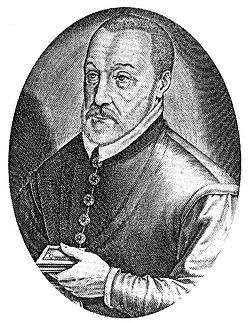
\includegraphics[width=0.85\textwidth]{../../images/python/page_030_img_01.jpeg}

\end{document}
